\documentclass[12pt,onecolumn]{article}


\usepackage{float}
\usepackage{mathtools}
\usepackage[russian]{babel}
\everymath{\displaystyle}

\usepackage[usenames]{color}
\usepackage{colortbl}

\usepackage{geometry}
\geometry{
  a4paper,
  top=15mm, 
  right=10mm, 
  bottom=15mm, 
  left=10mm
}

\begin{document}

\begin{center}
    Федеральное государственное автономное образовательное учреждение высшего образования\\
	«Национальный исследовательский университет ИТМО»
\end{center}
\vspace{1cm}


\begin{center}
    \large \textbf{Лабораторная работа №1}\\
    по дисциплине\\
    «ПРОГРАММИРОВАНИЕ»\\
	\vspace{1cm}
    Вариант №311805\\
\end{center}

\vspace{10cm}
\begin{flushright}
  Выполнил студент  группы P3118: \\
  \textbf{Кокорин Всеволод Вячеславович}\\
  Преподаватель: \\
  \textbf{Письмак Алексей Евгеньевич}\\
\end{flushright}

\vspace{5cm}
\begin{center}
    г. Санкт-Петербург\\
    2022г.
\end{center}
\newpage
\tableofcontents
\newpage
\section{Текст задания}
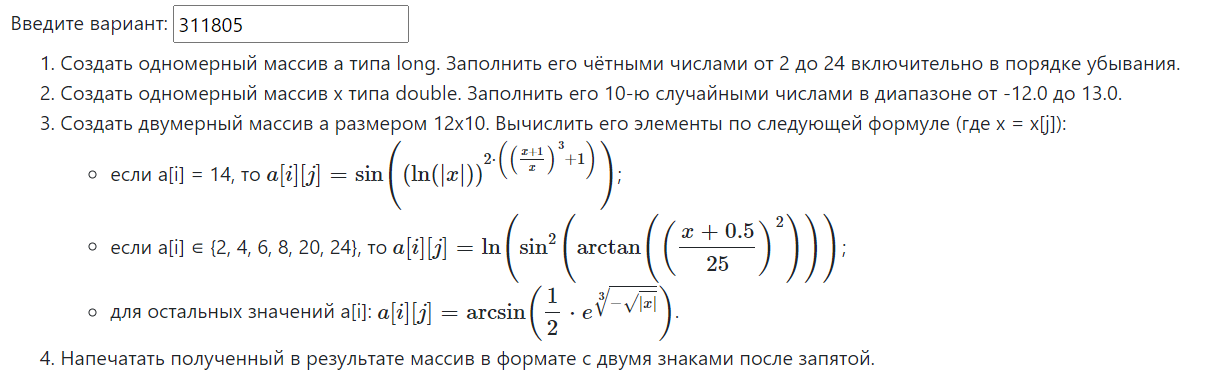
\includegraphics[width=\columnwidth]{img/task.png}

\newpage
\section{Исходный код программы}
https://github.com/Slonser/ITMO\_labs/tree/main/programming/lab1/src
\begin{center}
  
\includegraphics[width=7cm]{img/qr-code.png}
\end{center}

\newpage
\section{Результат выполнения}
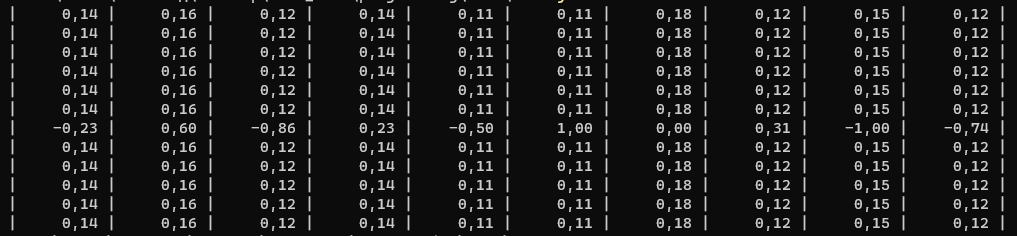
\includegraphics[width=\columnwidth]{img/result.png}

\newpage
\section{Вывод}
По ходу выполнения работы,  ознакомился с базовым синтаксисом языка Java. Научился пользоваться средствами разработки JDK и JRE. Познакомился с библиотекой java.lang.Math
\end{document}
